\documentclass[landscape, paperwidth=42in, paperheight=36in,
fontscale=.35, margin=1in]{baposter} 

% Packages to use
\usepackage{calc}
\usepackage{graphicx}
\usepackage{amsmath}
\usepackage{amssymb}
\usepackage{relsize}
\usepackage{multirow}
\usepackage{rotating}
\usepackage{bm}
\usepackage{enumitem}
\usepackage{url}
\usepackage{booktabs}
\usepackage{graphicx}
\usepackage{multicol}
\usepackage{tikz}
\usepackage[longnamesfirst]{natbib}
\usepackage{array}
\usepackage[T1]{fontenc}
% \usepackage[urw-garamond]{mathdesign}
% \usepackage{garamondx}

% Define colors
\definecolor{lightblue}{rgb}{0.145,0.6666,1}
\definecolor{darkblue}{rgb}{0.220,0.424,0.690}
\definecolor{lightred}{rgb}{0.81,0.2,.13}
\definecolor{darkred}{rgb}{0.8,0.18,0.15}
\definecolor{black}{rgb}{0,0,0}
\definecolor{dukeblue}{rgb}{0,0,0.612}

% Define custom commands
\newcommand{\compresslist}{%
\setlength{\itemsep}{1pt}%
\setlength{\parskip}{0pt}%
\setlength{\parsep}{0pt}%
}

% Begin poster and set options
\begin{document}
\begin{poster}{ 
  % Show grid to help with alignment
  grid=false,
  columns=3,
  % Column spacing
  colspacing=0.1in, 
  % Color style
  bgColorOne=white,
  bgColorTwo=white,
  borderColor=black,
  headerColorOne=dukeblue, % was black (gradient)
  headerColorTwo=dukeblue, % lightblue
  headerFontColor=white,
  boxColorOne=white,
  boxColorTwo=black, % lightblue
  % Format of textbox
  textborder=roundedleft,
  % Format of text header
  eyecatcher=true,
  headerborder=closed,
  headerheight=0.1\textheight,
%  textfont=\sc, An example of changing the text font
% headershape can be one of: rectangle, rounded, smallrounded, roundedleft, roundedright
  headershape=rounded, 
  headershade=shadelr,
  headerfont=\Large\bf\textsf, %Sans Serif 
  textfont={\setlength{\parindent}{1.5em}},
  boxshade=plain,
%  background=shade-tb,
  background=plain,
  linewidth=2pt
  } {%%% Eye Catcher %%%%%%%%
	\hspace{1.3in} 
        \setlength\fboxsep{0pt}
        \setlength\fboxrule{0.5pt}
        \fbox{
        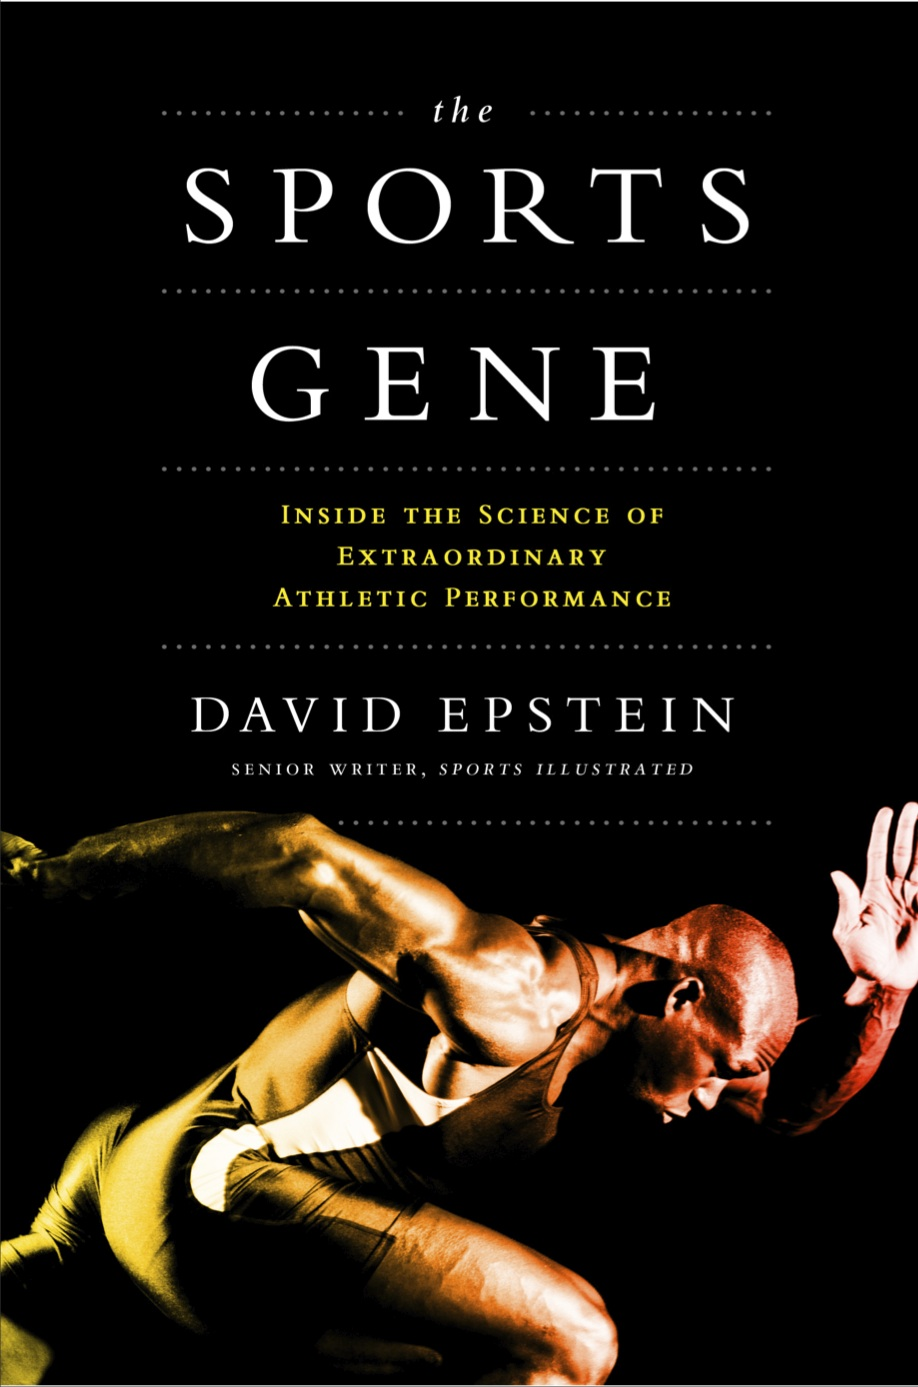
\includegraphics[scale=0.15]{../graphics/SportsGene.jpg}
        }
} {%%% Title %%%%%%%%
\textsf{
	\bf{Classifying Olympic Athletes By Sport}}
} { %%% Authors %%%%%%%
	\vspace{1em} \textsf{Matt Dickenson}\\
	{\smaller \textsf{mcd31@duke.edu}}
} {%%% Logo %%%%%%%%%%
  \centering 
\includegraphics[scale=.8]{dukelogo_vert_black.eps} \hspace{1in}
}


%%%%%%%%%%%%%%%%%%%%%%%%%%%%%%%%%%%%%%%%%%%%%%%%%%%%%%%%%%%%%%%%%%%%%%%%%%%%%%
%%% Now define the boxes that make up the poster
%%%---------------------------------------------------------------------------
%%% Each box has a name and can be placed absolutely or relatively.
%%% The only inconvenience is that you can only specify a relative position 
%%% towards an already declared box. So if you have a box attached to the 
%%% bottom, one to the top and a third one which should be in between, you 
%%% have to specify the top and bottom boxes before you specify the middle 
%%% box.
%%%%%%%%%%%%%%%%%%%%%%%%%%%%%%%%%%%%%%%%%%%%%%%%%%%%%%%%%%%%%%%%%%%%%%%%%%%%%%
    %
    % A coloured circle useful as a bullet with an adjustably strong filling
    \newcommand{\colouredcircle}{%
      \tikz{\useasboundingbox (-0.2em,-0.32em) rectangle(0.2em,0.32em); \draw[draw=black,fill=lightblue,line width=0.03em] (0,0) circle(0.18em);}}

%%%%%%
  \headerbox{\bf Motivation}{name=question,column=0,row=0}{
%%%%%
% Can political indicators such as the Militarized Interstate Dispute (MID) dataset be approximated by automated classification procedures? Existing, human-intensive pipelines for the production of MID and related data (e.g. Polity and Freedom House) are costly and slow. This project uses classification trees to estimate the MID occurrence using event data. 

To what extent do environmental or biological traits determine sporting success? At the highest level of amateur sports--the Olympic games--we can notice differences in the physical characteristics of participating athletes across sports. Can these differences be exploited to classify individuals by sport or event given their physical attributes? 
% If so, that suggests that athletes choose the event that best leverages their natural predisposition. If not, this implies that athletic ability is best understood as a latent trait that can be applied to the sport of one's choice.

This project was inspired by a claim made by David Epstein, author of \textit{The Sports Gene}. This claim is expressed in an interview with Russ Roberts:
\begin{quote}
\footnotesize
\textbf{Roberts}: [You argue that] if you simply had the height and weight of an Olympic roster, you could do a pretty good job of guessing what their events are. Is that correct? \\
\textbf{Epstein}: That's definitely correct. I don't think you would get every person accurately, but... \textit{I think you would get the vast majority of them correctly.} And frankly, you could definitely do it easily if you had them charted on a height-and-weight graph, and I think you could do it for most positions in something like football as well.
\end{quote}

 }

%%%%%%
  \headerbox{\bf Data}{name=data,below=question}{
%%%%%
  Data was obtained for participants in the 2012 London Olympics from \textit{The Guardian}. The original data consisted of 10,383 participants, which was reduced to 6,956 observations after data processing. The processed data was randomly split into training ($n$=3,520) and test ($n$=3,436). Athletes' height, weight, and age were used as features to predict their Olympic sport. Some sports exhibit relatively well-clustered features, whereas others are more scattered.

  \begin{center}
  %   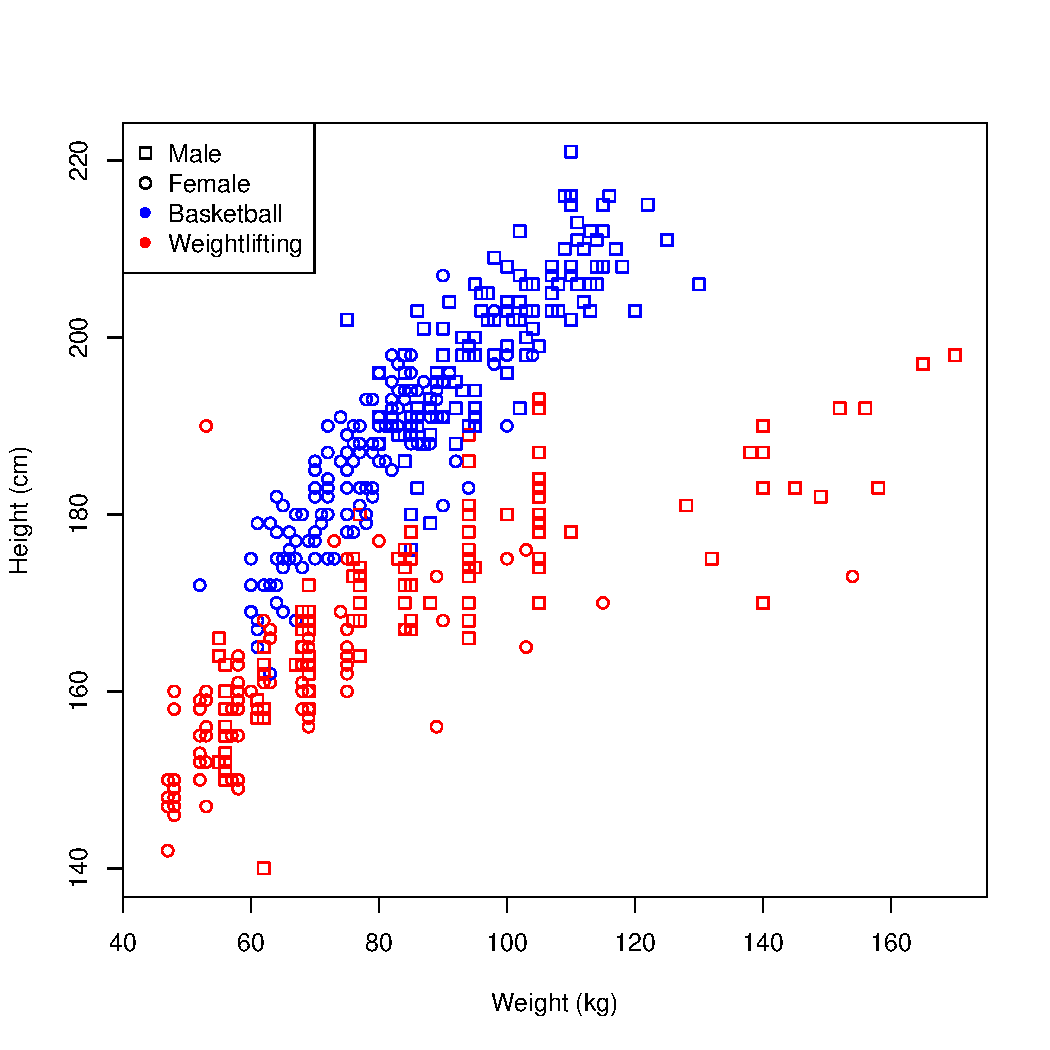
\includegraphics[scale=0.27]{../graphics/Basketball-Weightlifting.pdf}
  % \end{center}

  \begin{minipage}{0.45\textwidth}
    \begin{center}
      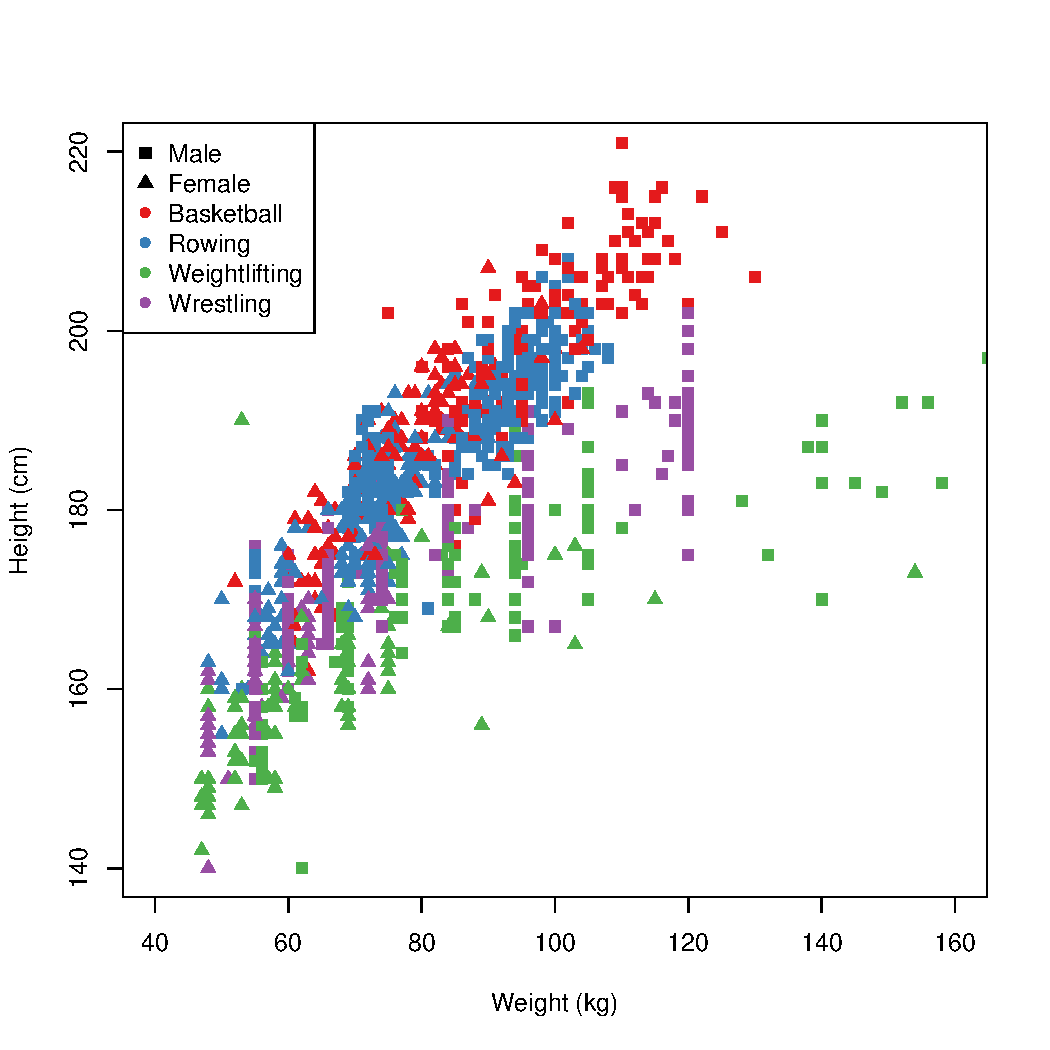
\includegraphics[scale=0.27]{../graphics/basketball.pdf}
    \end{center}
  \end{minipage}
  \hspace{0.05\textwidth}
  \begin{minipage}{0.45\textwidth}
    \begin{center}
      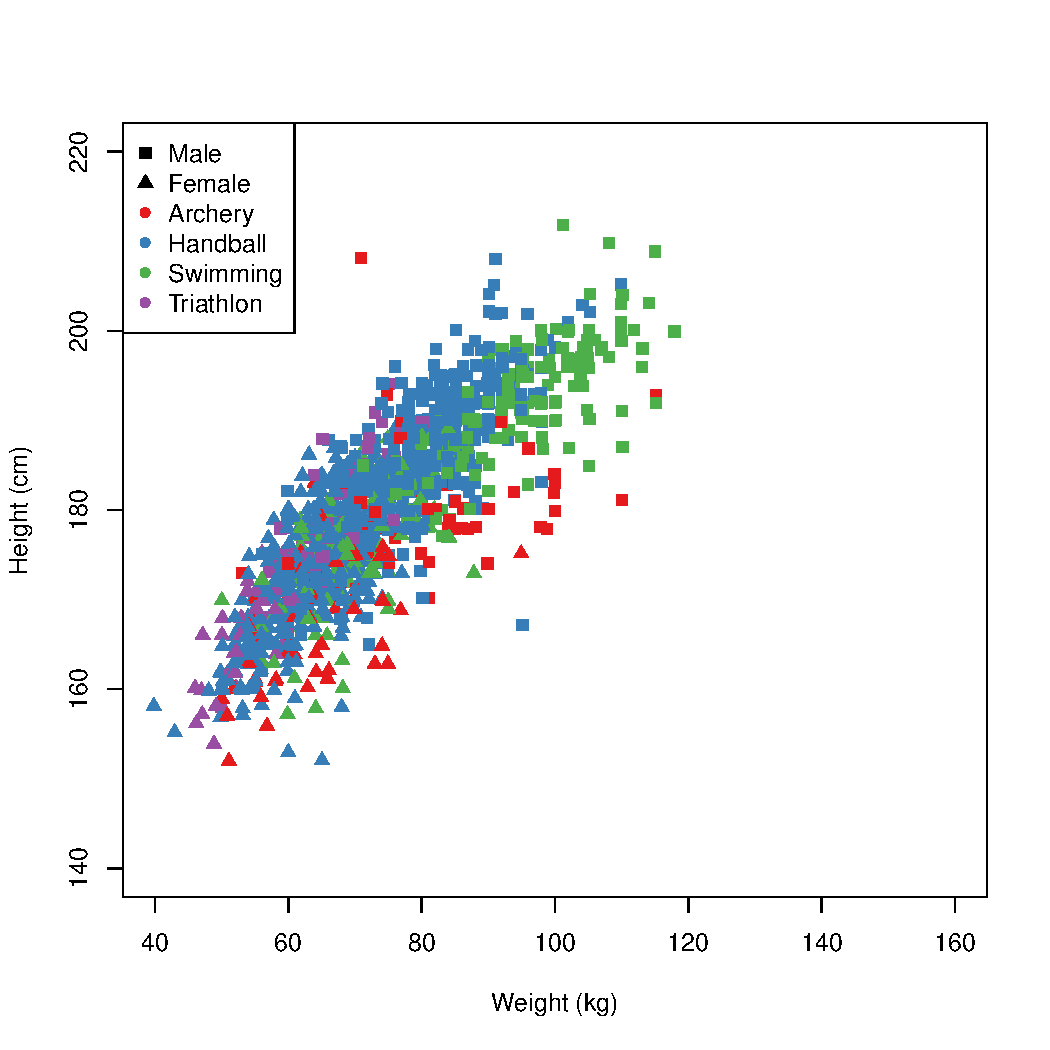
\includegraphics[scale=0.27]{../graphics/swimming.pdf}
    \end{center}
  \end{minipage}
  \end{center}
 }

%%%%%%
  \headerbox{\bf Methodology}{name=methods,below=data,above=bottom}{
%%%%%
  Several machine learning methods were applied to this classification problem. Hierarchical clustering using Gaussian marginal likelihoods was performed using the \texttt{mclust} package.
  % todo: list methods here (and maybe R packages?)

  \begin{center}
  \footnotesize
    \begin{tabular}{lccc}
       \multicolumn{1}{c}{} & \multicolumn{1}{c}{Training Accuracy} & \multicolumn{1}{c}{Test Accuracy} & \multicolumn{1}{c}{Ratio} \\
      \midrule
      \footnotesize{Hierarchical Clustering}     & .272 & .271 & .998 \\
      \footnotesize{Conditional Inference Tree}  & .279 & .219 & .784 \\
      \footnotesize{Evolutionary Tree}           & .292 & .236 & .807 \\
      \footnotesize{Random Forest}               & .923 & .244 & .265 \\
      \footnotesize{Neural Network}              & .280 & .265 & .949 
    \end{tabular}
  \end{center}

  % The next column presents these results visually, with row-normalized observed frequencies. The figure below serves as a legend for all heatmaps.

  % \begin{center}
  %   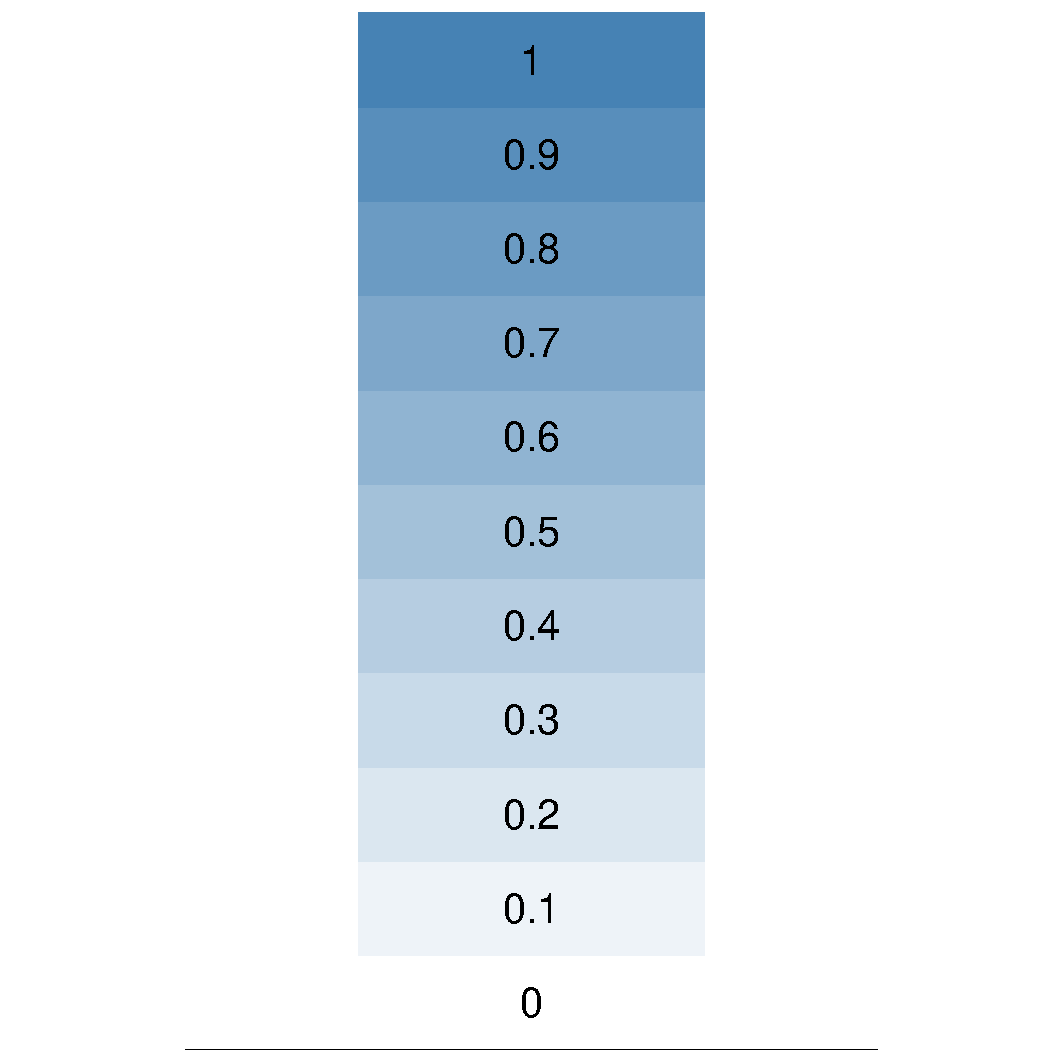
\includegraphics[scale=0.2]{../graphics/scale.pdf}
  % \end{center}

  \begin{minipage}{0.45\textwidth}
    The next column presents these results visually, with row-normalized observed frequencies. The figure at right serves as a legend for all heatmaps.
  \end{minipage}
  \hspace{0.05\textwidth}
  \begin{minipage}{0.45\textwidth}
    \begin{center}
      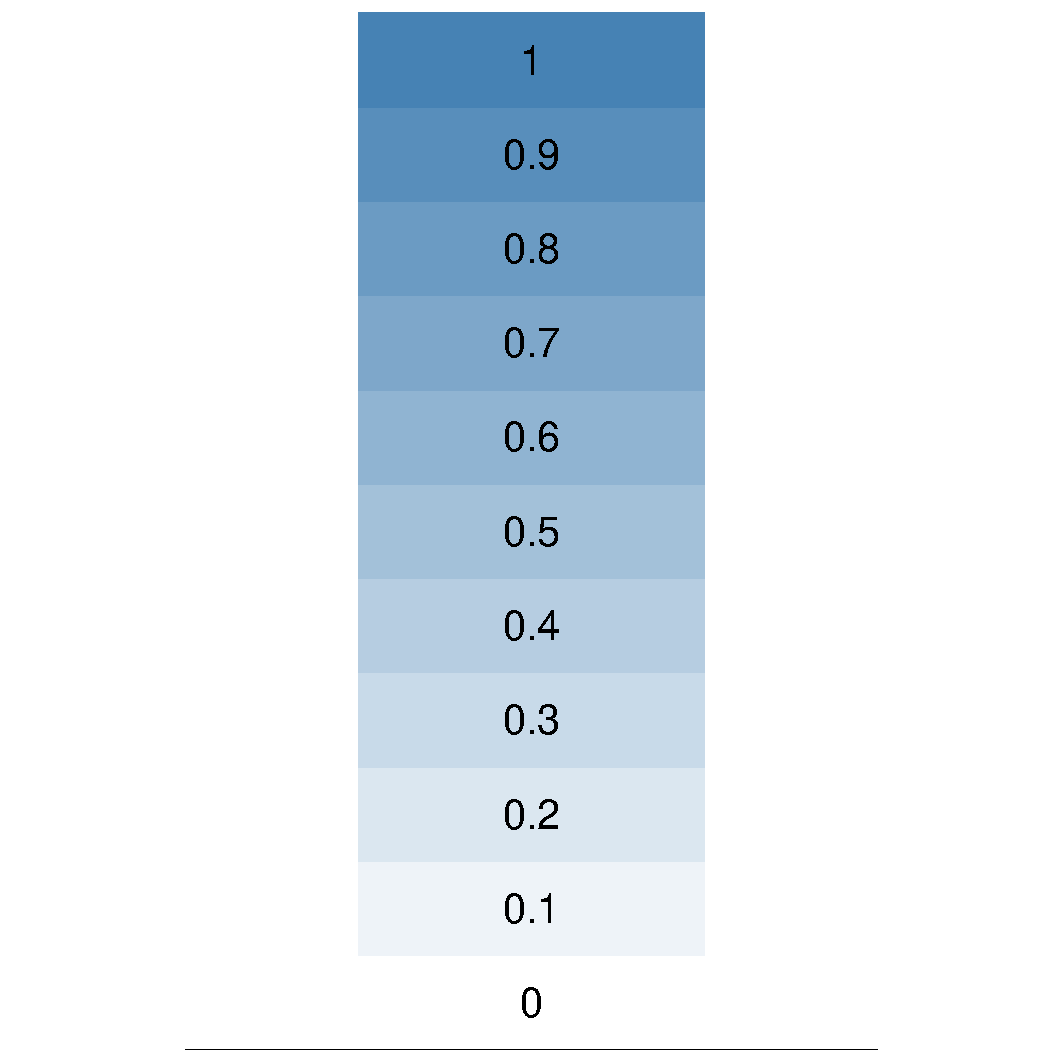
\includegraphics[scale=0.2]{../graphics/scale.pdf}
    \end{center}
  \end{minipage}
 }


%%%%%%
  \headerbox{\bf Results}{name=estimations,column=1,row=0}{
%%%%%

  \begin{center}
  %%%%%%%%%%%%%%%%%%%%%%%%%%%%%%%%%%%%%%%%%%%%%%%%%%%%%%%%%
  Hierarchical Clustering \\
  \begin{minipage}{0.45\textwidth}
    \begin{center}
      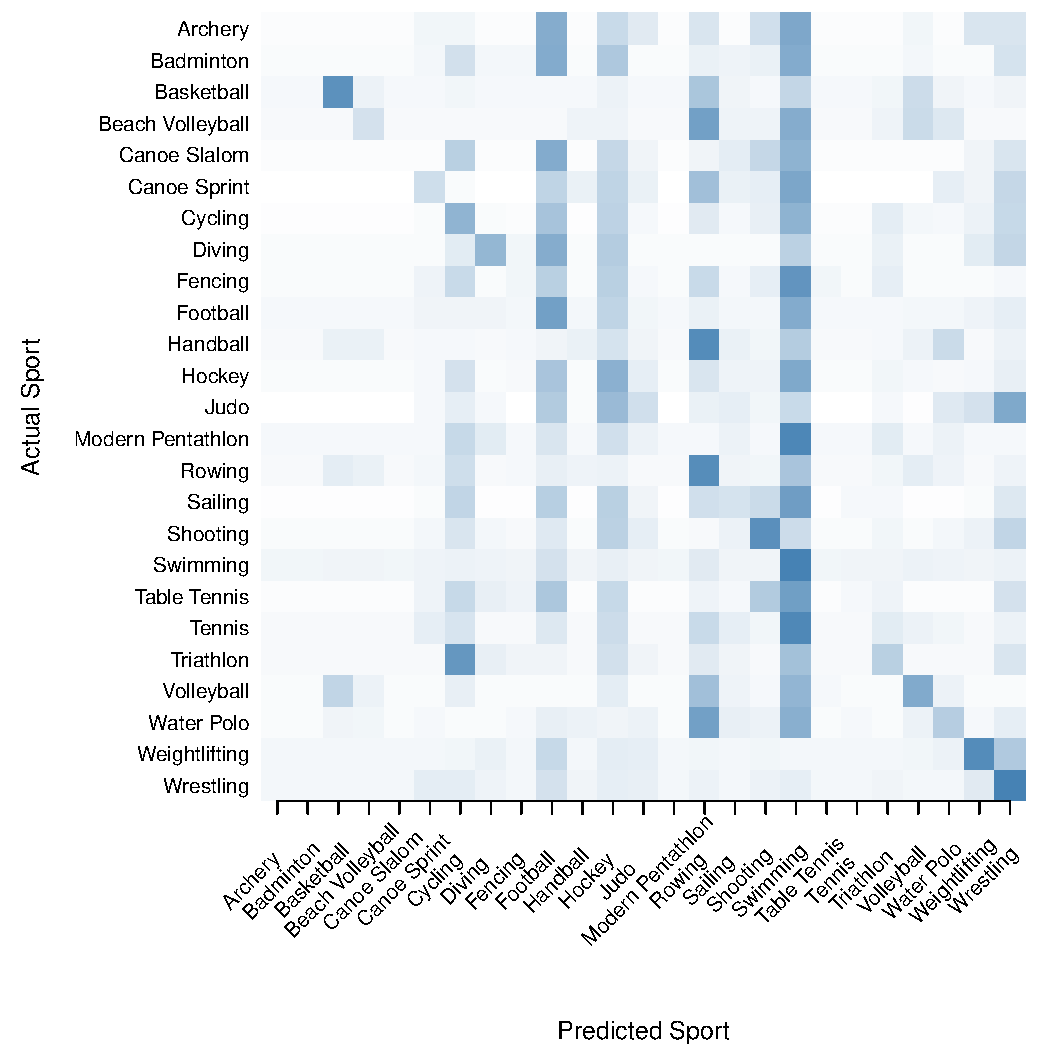
\includegraphics[scale=0.27]{../graphics/sportMclust-trn.pdf}
    \end{center}
  \end{minipage}
  \hspace{0.05\textwidth}
  \begin{minipage}{0.45\textwidth}
    \begin{center}
      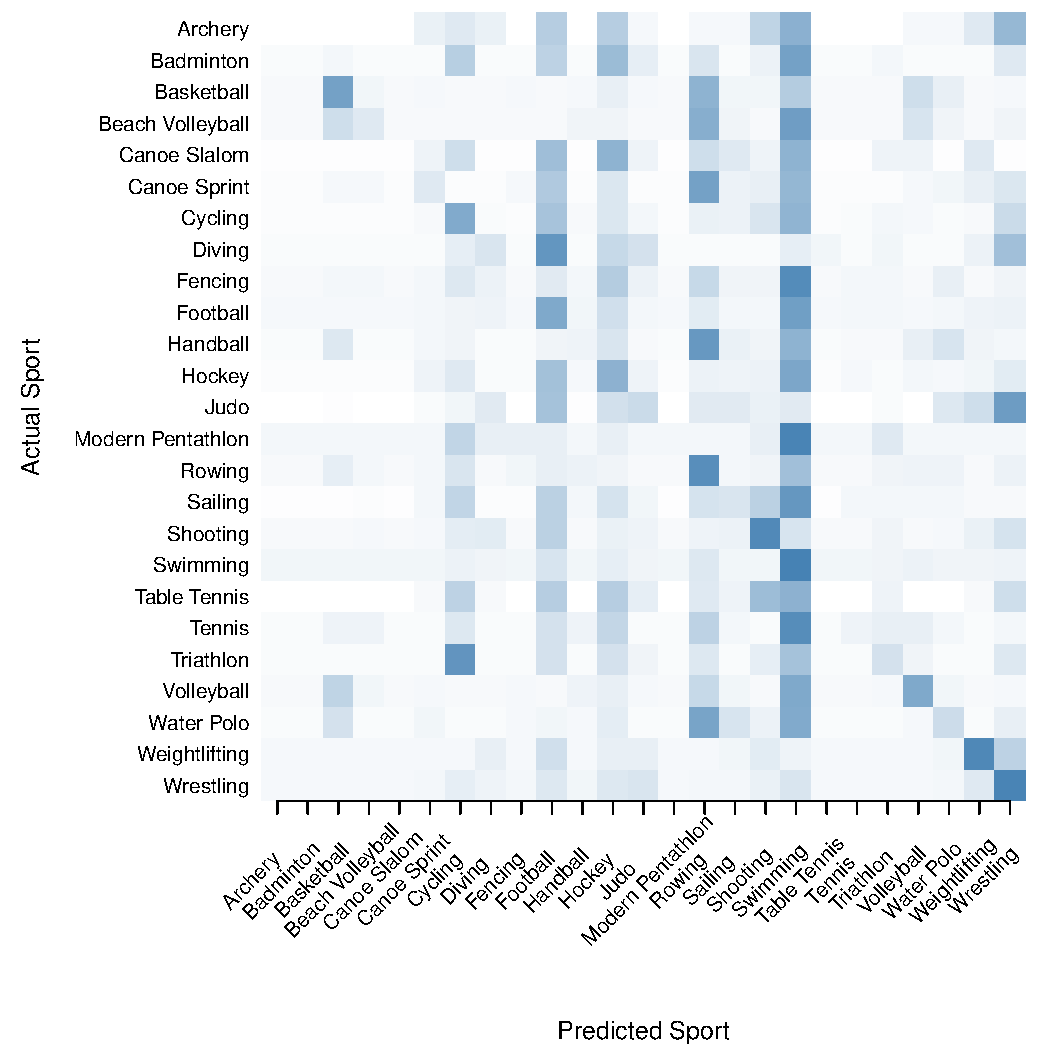
\includegraphics[scale=0.27]{../graphics/sportMclust-tst.pdf}
    \end{center}
  \end{minipage}


  %%%%%%%%%%%%%%%%%%%%%%%%%%%%%%%%%%%%%%%%%%%%%%%%%%%%%%%%%
  Conditional Inference Tree \\
  \begin{minipage}{0.45\textwidth}
    \begin{center}
      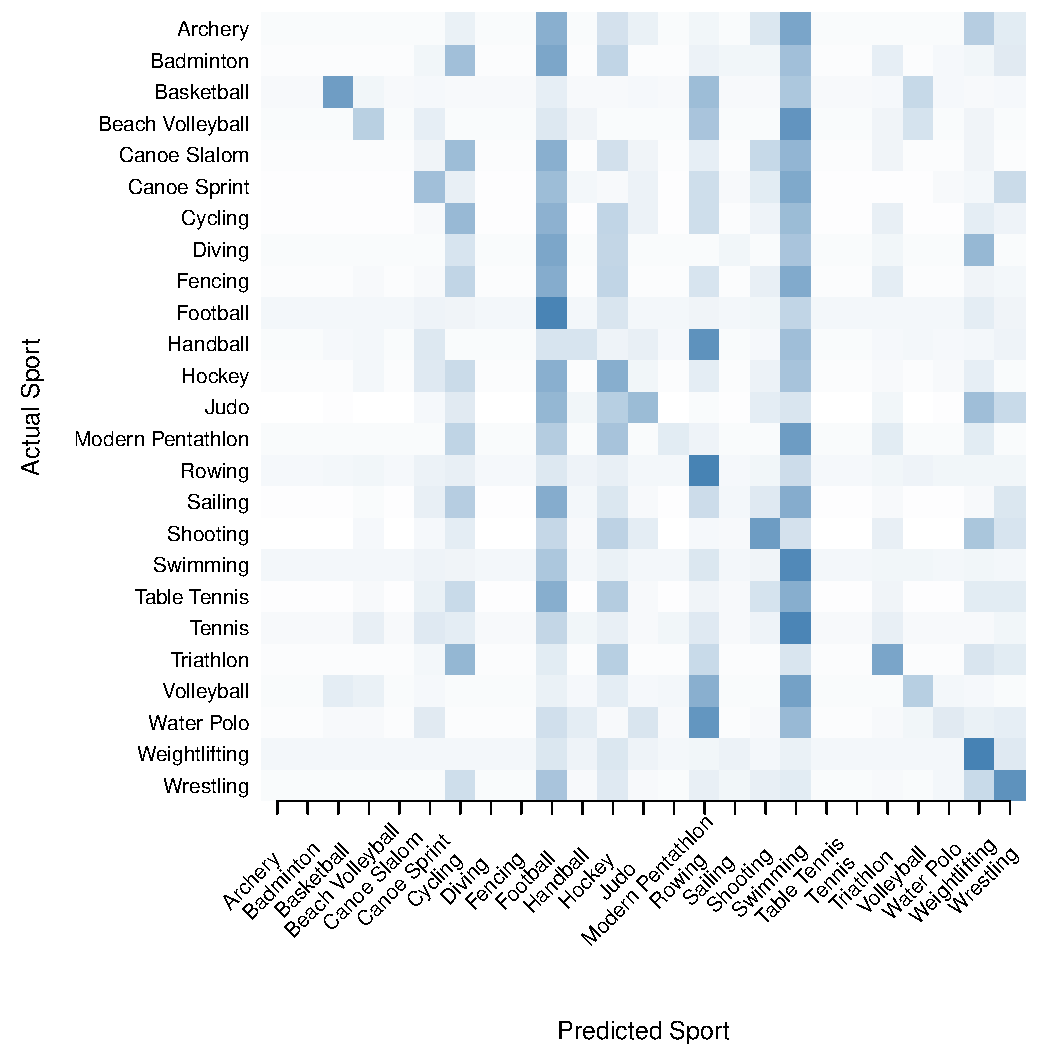
\includegraphics[scale=0.27]{../graphics/sportCIT-trn.pdf}
    \end{center}
  \end{minipage}
  \hspace{0.05\textwidth}
  \begin{minipage}{0.45\textwidth}
    \begin{center}
      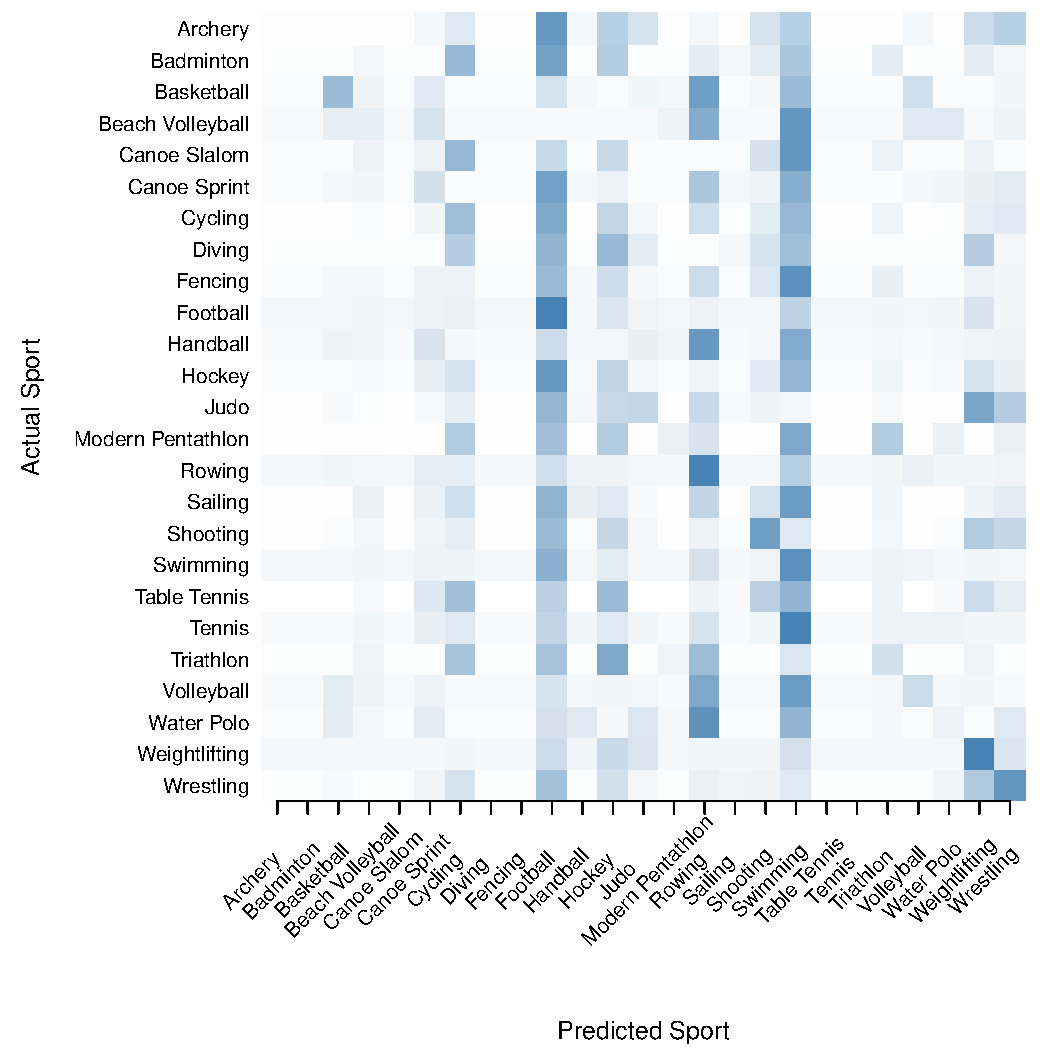
\includegraphics[scale=0.27]{../graphics/sportCIT-tst.pdf}
    \end{center}
  \end{minipage}


  %%%%%%%%%%%%%%%%%%%%%%%%%%%%%%%%%%%%%%%%%%%%%%%%%%%%%%%%%
  Evolutionary Tree \\
  \begin{minipage}{0.45\textwidth}
    \begin{center}
      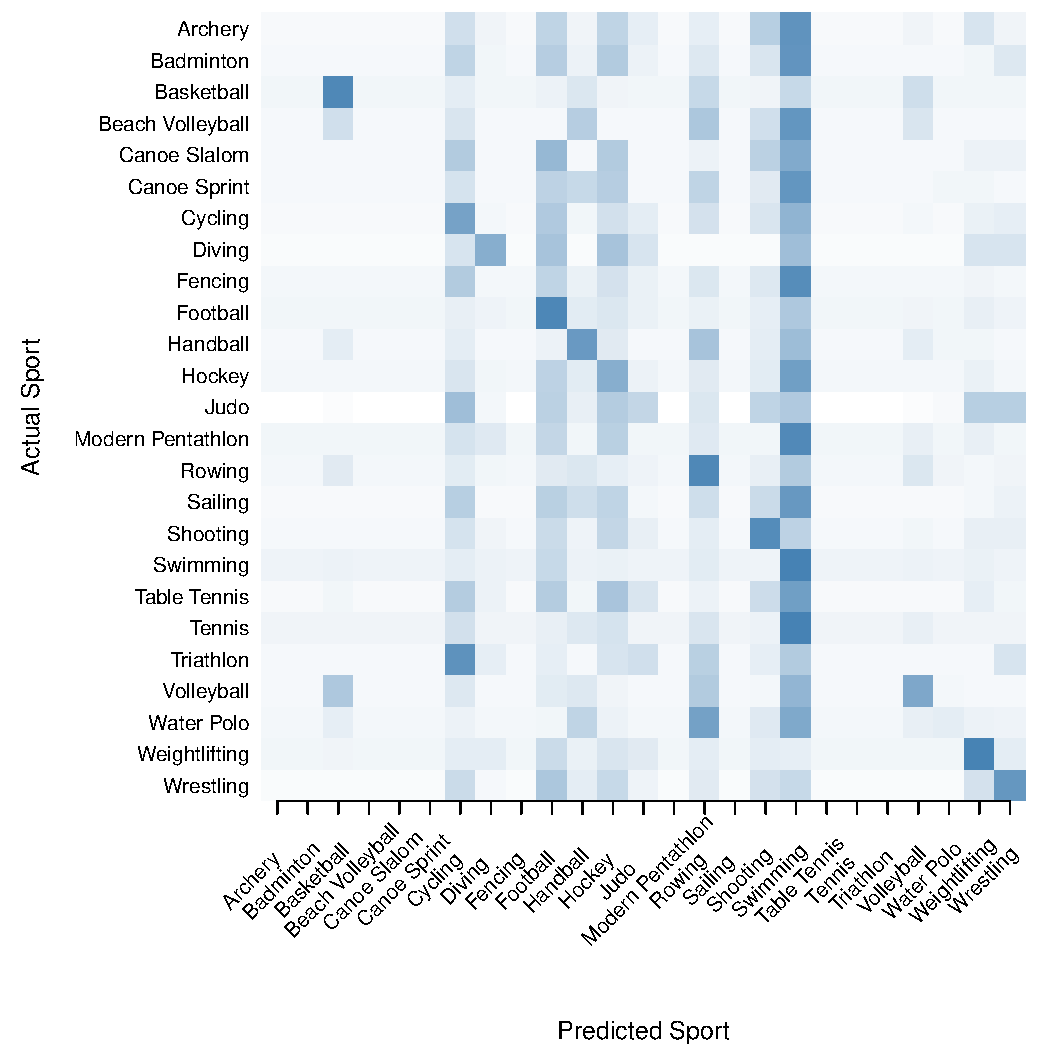
\includegraphics[scale=0.27]{../graphics/sportEV-trn.pdf}
    \end{center}
  \end{minipage}
  \hspace{0.05\textwidth}
  \begin{minipage}{0.45\textwidth}
    \begin{center}
      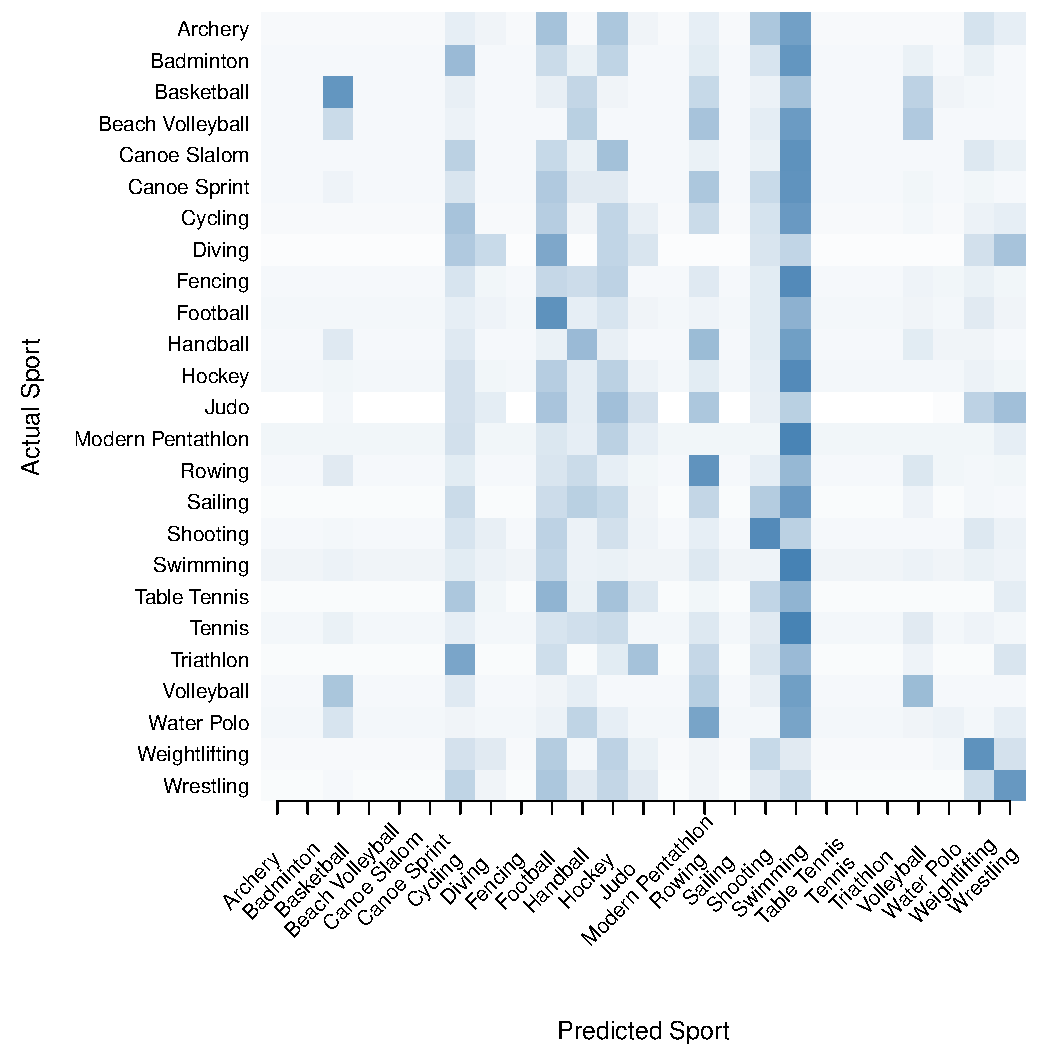
\includegraphics[scale=0.27]{../graphics/sportEV-tst.pdf}
    \end{center}
  \end{minipage}


  %%%%%%%%%%%%%%%%%%%%%%%%%%%%%%%%%%%%%%%%%%%%%%%%%%%%%%%%%
  Random Forest \\
  \begin{minipage}{0.45\textwidth}
    \begin{center}
      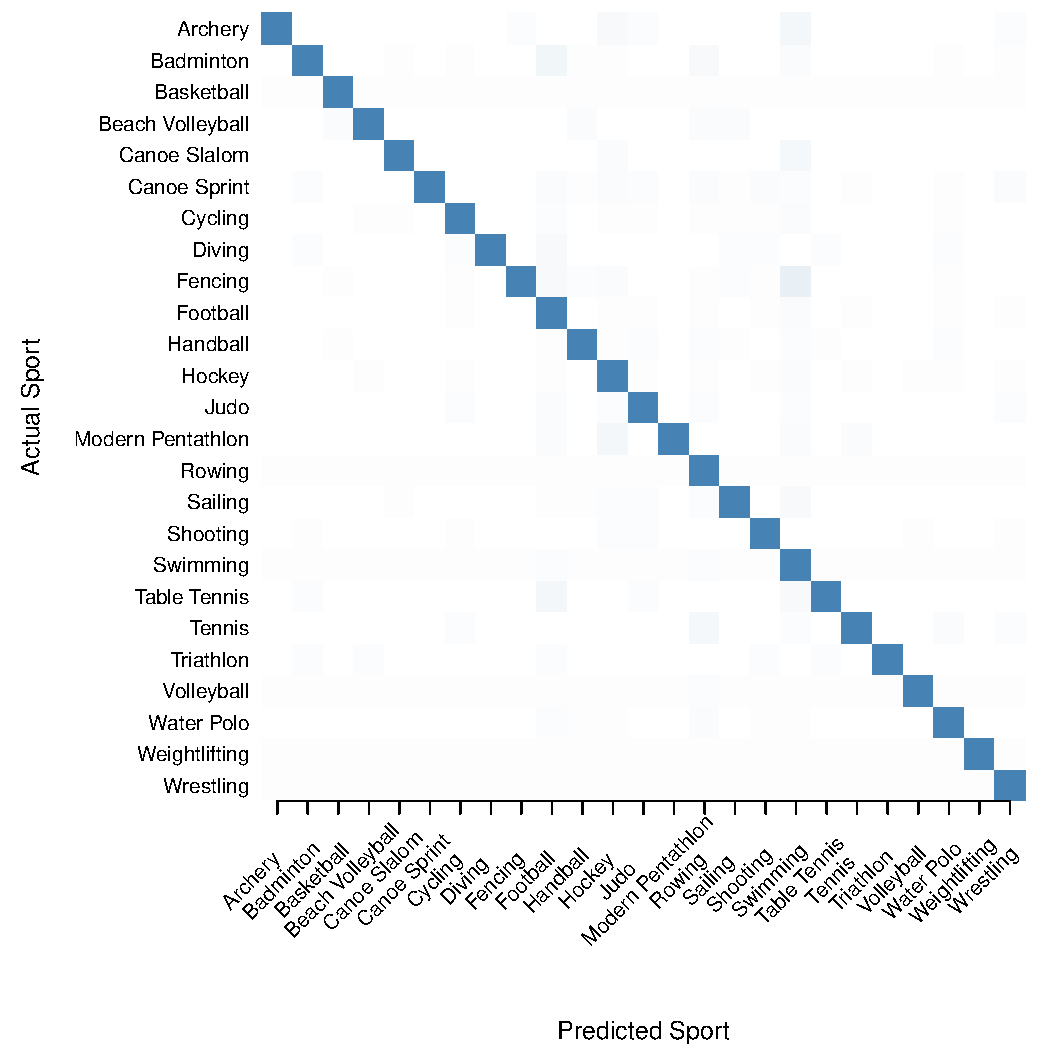
\includegraphics[scale=0.27]{../graphics/sportRF-trn.pdf}
    \end{center}
  \end{minipage}
  \hspace{0.05\textwidth}
  \begin{minipage}{0.45\textwidth}
    \begin{center}
      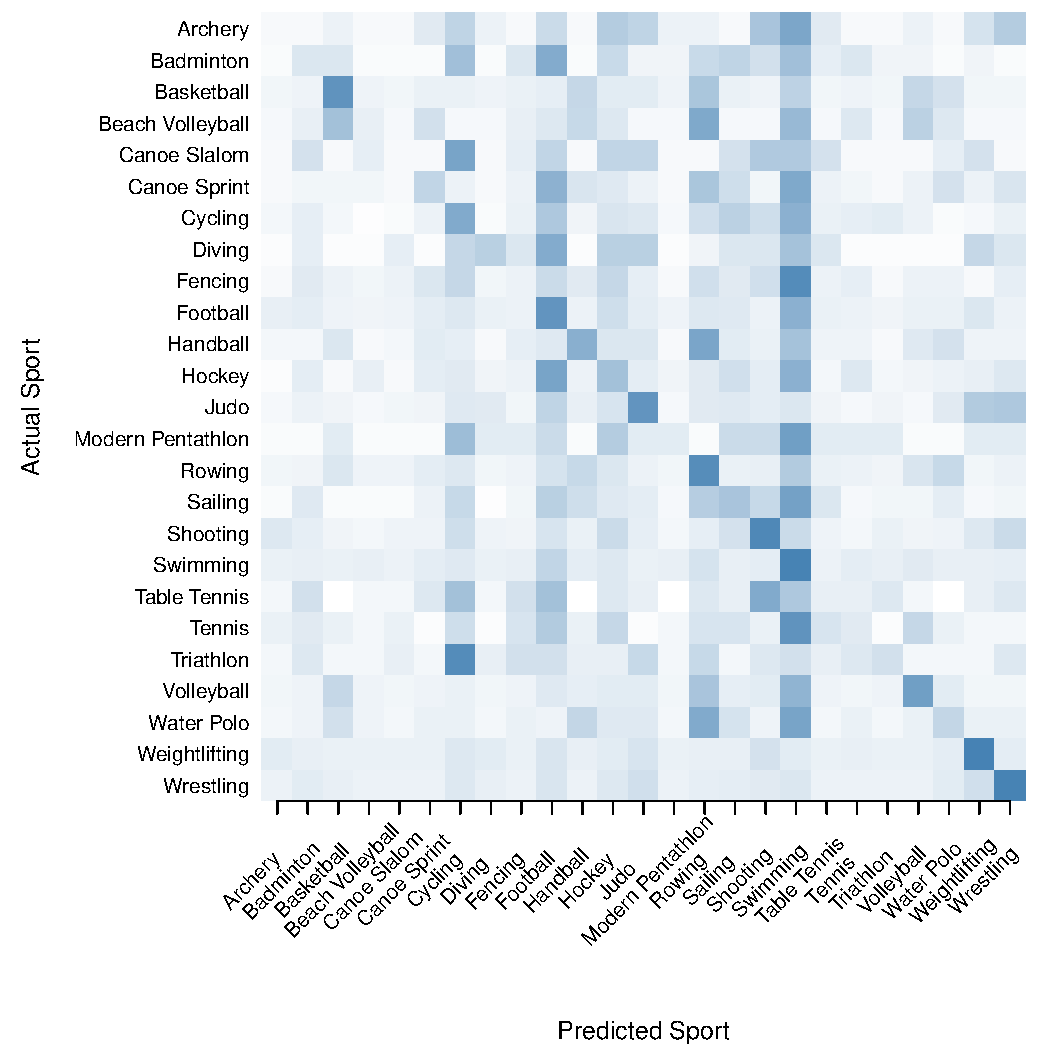
\includegraphics[scale=0.27]{../graphics/sportRF-tst.pdf}
    \end{center}
  \end{minipage}


  %%%%%%%%%%%%%%%%%%%%%%%%%%%%%%%%%%%%%%%%%%%%%%%%%%%%%%%%%
  Neural Network \\
  \begin{minipage}{0.45\textwidth}
    \begin{center}
      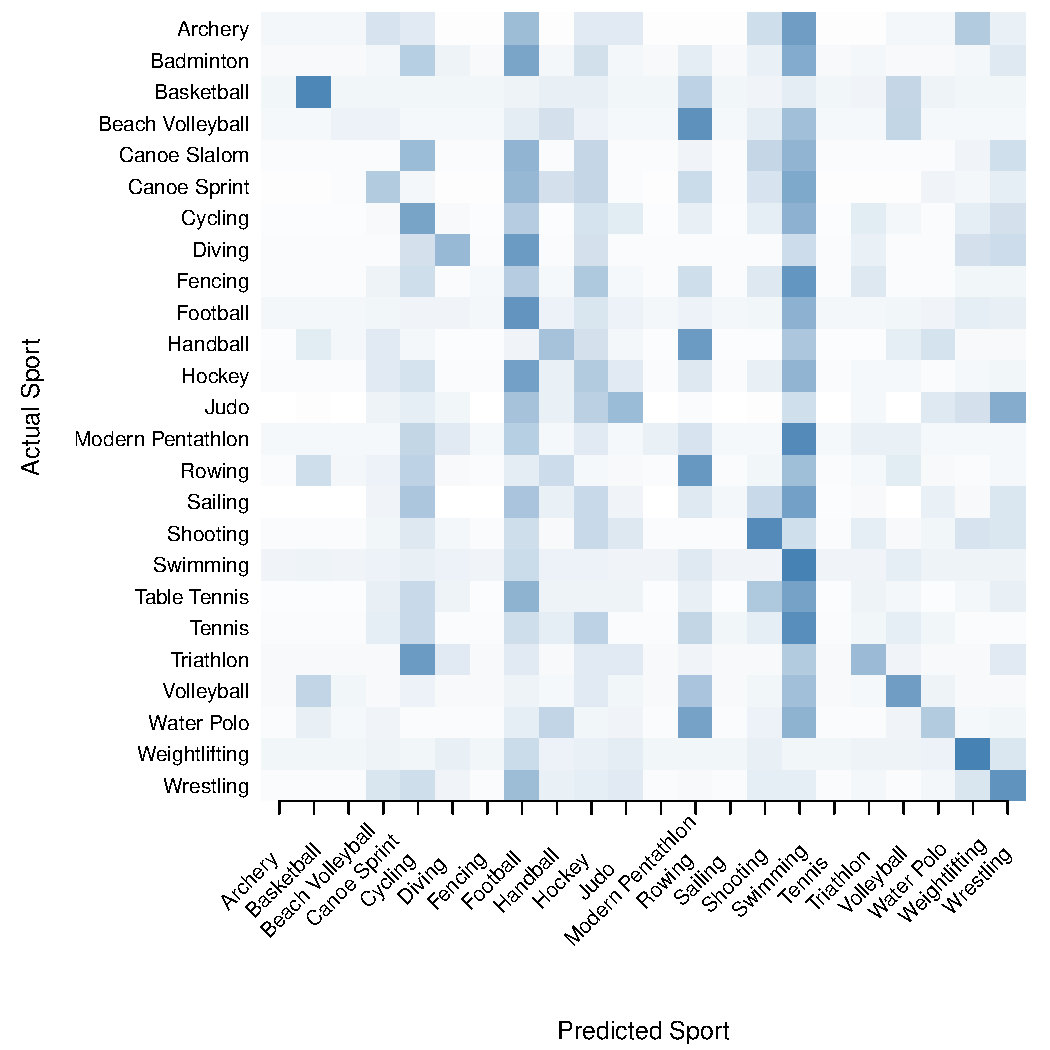
\includegraphics[scale=0.27]{../graphics/sportANN-trn.pdf}
    \end{center}
  \end{minipage}
  \hspace{0.05\textwidth}
  \begin{minipage}{0.45\textwidth}
    \begin{center}
      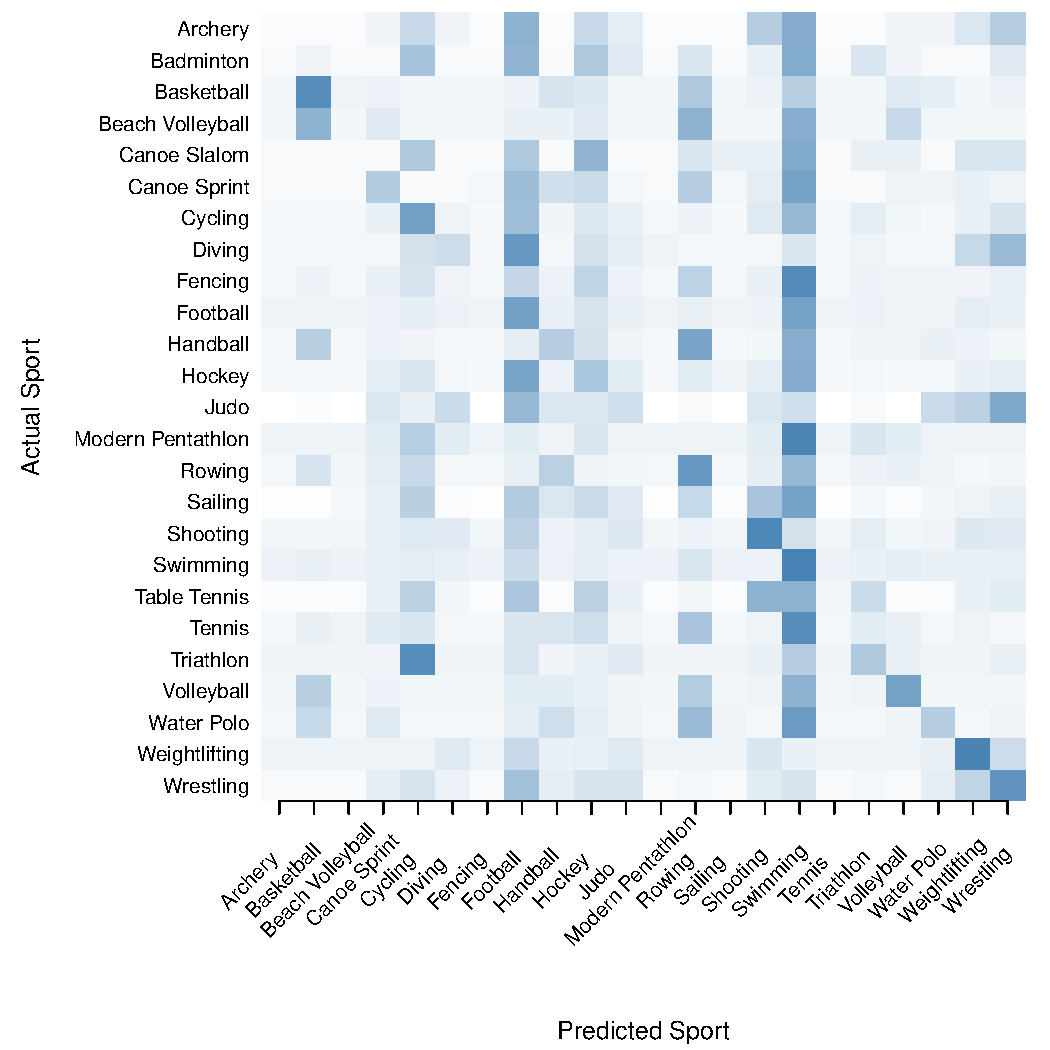
\includegraphics[scale=0.27]{../graphics/sportANN-tst.pdf}
    \end{center}
  \end{minipage}
  \end{center}



 }


%%%%%%
  \headerbox{\bf Results}{name=predictions,column=2,row=0}{
%%%%%
  
    \begin{center}
      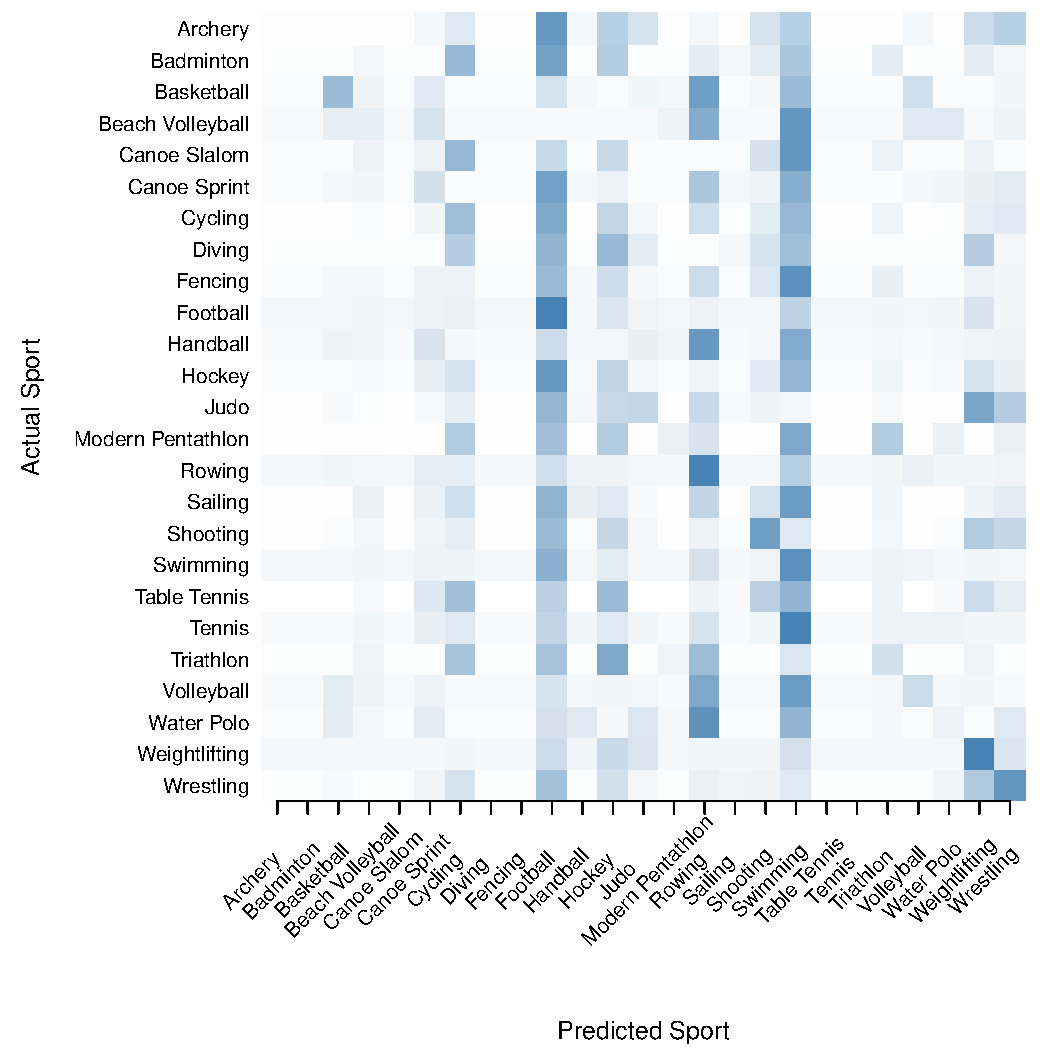
\includegraphics[scale=0.2]{../graphics/sportCIT-tst.pdf}
    \end{center}

 }

%%%%%%
  \headerbox{\bf Discussion}{name=conclusion,below=predictions,above=bottom,column=2}{
%%%%%
   \begin{itemize} \compresslist
      \item Classifying athletes by sport can be achieved with moderate accuracy using only a few features
      \item Classification with a large number of categories is difficult
      \item Traits of athletes in some sports exhibit noticeable clustering, while other clusters are less distinct (multi-modal)
      \item Athletes in some sports have a well-defined body type, but athletes exhibit a wide range of physical features
  \end{itemize}
 }

\end{poster}
\end{document}